\documentclass{standalone}
\usepackage{tikz}
\begin{document}
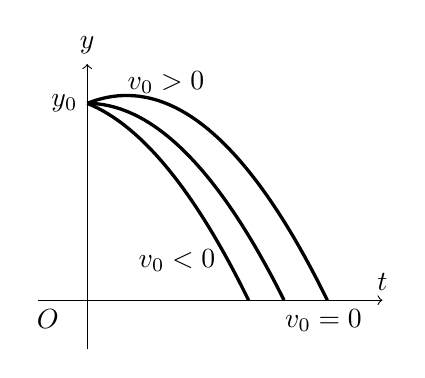
\begin{tikzpicture}[scale = 2.5]
    \coordinate (O) at (0,0);
    \node[left] at (0, 1) {$y_0$};
    \node[below] at (1.2, 0) {$v_0 = 0$};
    \node[above] at (.4, 1) {$v_0 > 0$};
    \node[left] at (0.7, 0.2) {$v_0 < 0$};
    \draw[-,very thick] plot[smooth, domain=0:0.82] (\x, {1.04 - (\x + .2)^2});
    \draw[-,very thick] plot[smooth, domain=0:1] (\x, {1-(\x)^2});
    \draw[-,very thick] plot[smooth, domain=0:1.22] (\x, {1.04-(\x - .2)^2});
    \node[below] at (-0.2,0) {$O$};
    \draw[->] (-0.25, 0) -- (1.5, 0) coordinate (t) node[above]{$t$};
    \draw[->] (0,-0.25) --(0,1.2) coordinate (y) node[above]{$y$};
\end{tikzpicture}
\end{document}